\documentclass{article}

% Environment setup

\usepackage[
    margin=1in
]{geometry} %geometry (sets margin) and other useful packages 
% \setlength{\oddsidemargin}{.25in}
% \setlength{\evensidemargin}{.25in}
% \setlength{\textwidth}{6in}
% \addtolength{\topmargin}{-0.4in}
% \setlength{\textheight}{8.5in}
\setlength{\parindent}{0em}
\setlength{\parskip}{.75em}

\usepackage{graphicx}
\usepackage{grffile}  % support extra dots in filenames
\usepackage{fancyref}
\usepackage[labelfont=bf]{caption}
\usepackage{subcaption}


\title{\textbf{CS 4641:} Randomized Optimization}
\author{Bradley Reardon}
\date{March 3, 2019}

\begin{document}
  \maketitle

  \section{Introduction}
    The purpose of this assignment is to evaluate various random search algorithms. Namely, the algorithms of interest that will be explored in this report are: randomized hill climbing, simulated annealing, genetic algorithms, and MIMIC.

    The first part of this report will focus on using random hill climbing, simulated annealing, and genetic algorithms to optimize the weights for a neural network. The second part, on the other hand, focuses on distinguishing the strengths of the simulated annealing, genetic algorithm, and MIMIC algorithms by applying each in the context of various well-known optimization problems.

    \textbf{TODO more intro?}

  \section{Optimizing Neural Network Weights}

    \subsection{Introduction}
      In this section, we will use implementations of the randomized hill climbing, simulated annealing, and genetic algorithms in the ABAGAIL source code provided along with the assignment to optimize the weights of a neural network. We will first focus on sensible parameter selection where required to determine an optimial configuration for each of the algorithms. Then, we will evaluate the performance of the algorithms both individually and collectively on the breast cancer data set used in the previous assignment.

      \textbf{TODO: neural network params, 5 hidden layer, 1000 iter}

      \subsubsection{Breast Cancer Wisconsin data set}
        The Breast Cancer Wisconsin data set was donated to the UCI Machine Learning Repository in 1992, and contains data from one doctor's clinical cases, gathered from January 1989 to November 1991. In total, there are 699 instances signifying information about breast tumors such as clump thickness, uniformity in shape and size, and other screening factors. Data points are identified by two classes -- benign or malignant. The features of the data points are encoded as 9 continuous attributes rating the screening factor from 1 to 10.

        This data set contains unknowns in the form of question marks in the data. Due to the nature of the implementations in ABAGAIL, these 16 data points containing unknowns were stripped from the data set. Therefore, the set used for this report contains 683 instances.

        The problem at hand for this data set is determining whether a tumor is benign or malignant based on tumor screening characteristics identified in the data set.

        \textbf{Source:} https://archive.ics.uci.edu/ml/datasets/Breast+Cancer+Wisconsin+\%28Original\%29

    \subsection{Randomized Hill Climbing}

      \subsubsection{Parameter selection}
        TODO

        \Fref{fig:rhc-params} shows the training and test error curves for the cancer data set using randomized hill climbing for weight optimization. Each bar represents the training and test error at iteration \#1000 for varying numbers of restarts.

        \begin{figure}[htb]
        \centering

        \begin{subfigure}{0.5\textwidth}
          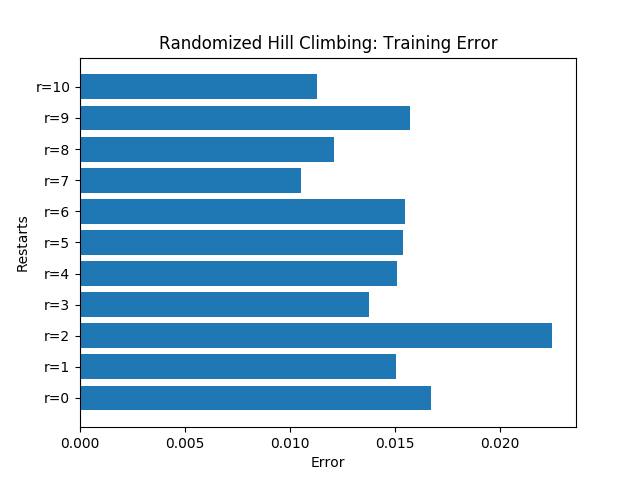
\includegraphics[width=\linewidth]{out/rhc/restarts-training.png}
          \caption{Training error}
          \label{fig:rhc-params-1}
        \end{subfigure}\hfil
        \begin{subfigure}{0.5\textwidth}
          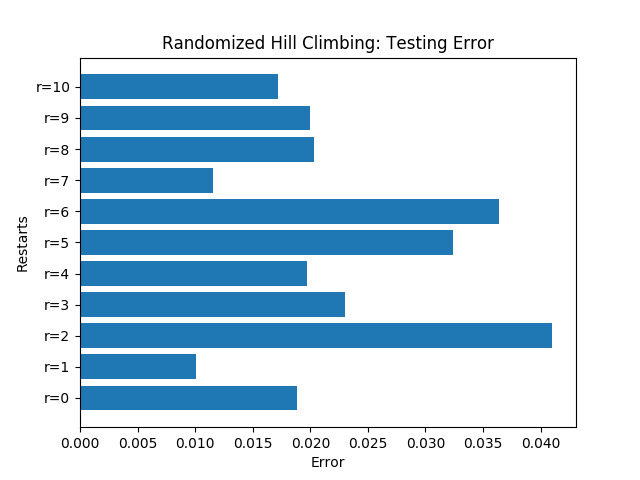
\includegraphics[width=\linewidth]{out/rhc/restarts-testing.png}
          \caption{Testing error}
          \label{fig:rhc-params-2}
        \end{subfigure}

        \caption{Learning curves for randomized hill climbing with varying restarts.}
        \label{fig:rhc-params}
        \end{figure}

        TODO TODO

      \subsubsection{Evaluation}
        \Fref{fig:rhc-learning} shows the learning curves for the cancer data set, using randomized hill climbing with no restarts.

        \begin{figure}[htb]
        \centering
        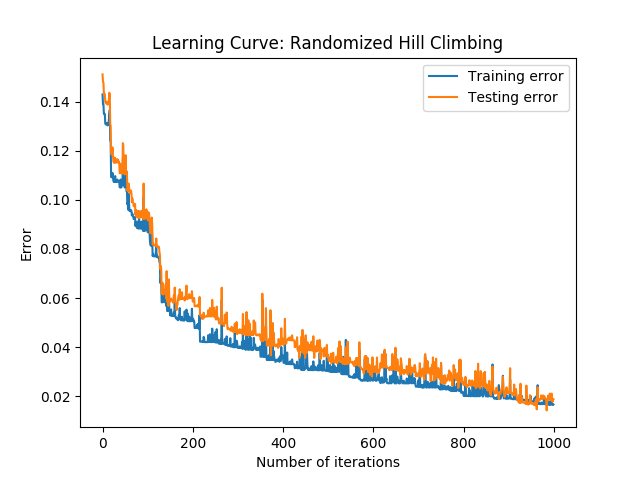
\includegraphics[width=.5\linewidth]{out/plot/RHC.png}
        \caption{Learning curve for random hill climbing.}
        \label{fig:rhc-learning}
        \end{figure}

    \subsection{Simulated Annealing}

      \subsubsection{Parameter selection}
        \Fref{fig:sa-params} shows the training and test error curves for the cancer data set using simulated annealing for weight optimization. The different series in the figure represent different cooling rates.

        \begin{figure}[htb]
        \centering

        \begin{subfigure}{0.5\textwidth}
          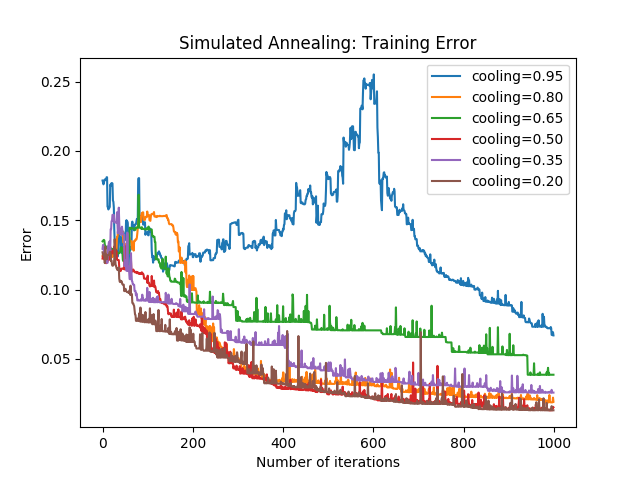
\includegraphics[width=\linewidth]{out/sa/cooling-error-training.png}
          \caption{Training error}
          \label{fig:sa-params-1}
        \end{subfigure}\hfil
        \begin{subfigure}{0.5\textwidth}
          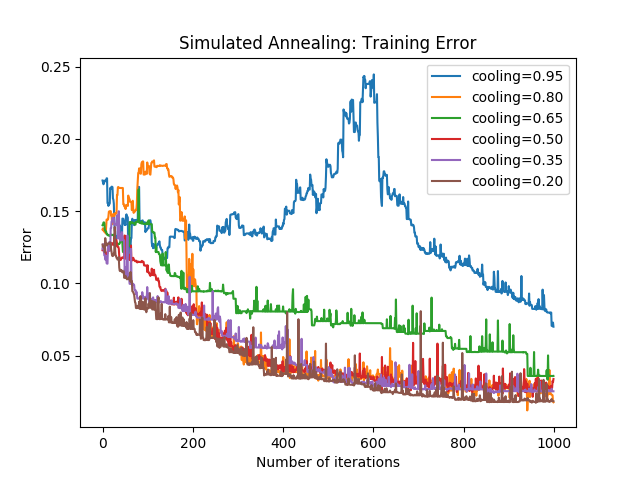
\includegraphics[width=\linewidth]{out/sa/cooling-error-testing.png}
          \caption{Testing error}
          \label{fig:sa-params-2}
        \end{subfigure}

        \caption{Learning curves for simulated annealing with different cooling rates.}
        \label{fig:sa-params}
        \end{figure}

        Select cooling rate of 0.20, lowest variance and lowest error soonest

        TODO TODO

      \subsubsection{Evaluation}
        \Fref{fig:sa-learning} shows the learning curves for the cancer data set using simulated annealing.

        \begin{figure}[htb]
        \centering
        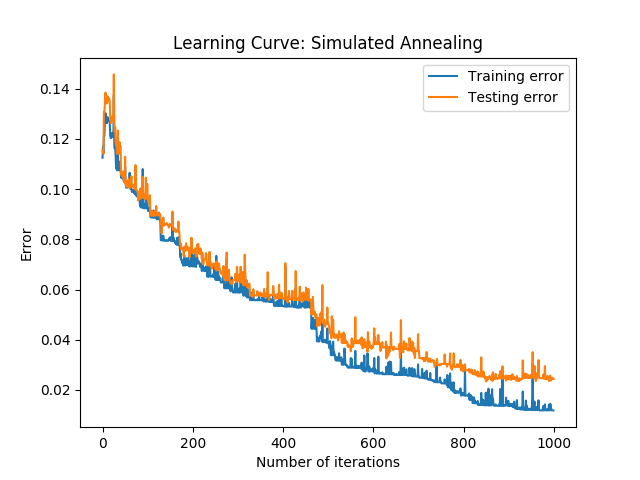
\includegraphics[width=.5\linewidth]{out/plot/SA.png}
        \caption{Learning curve for simulated annealing.}
        \label{fig:sa-learning}
        \end{figure}

    \subsection{Genetic Algorithms}

      \subsubsection{Parameter selection}
        \Fref{fig:ga-population} shows the training and test error curves for the cancer data set using genetic algorithms for weight optimization, varying the population size.

        \begin{figure}[htb]
        \centering

        \begin{subfigure}{0.5\textwidth}
          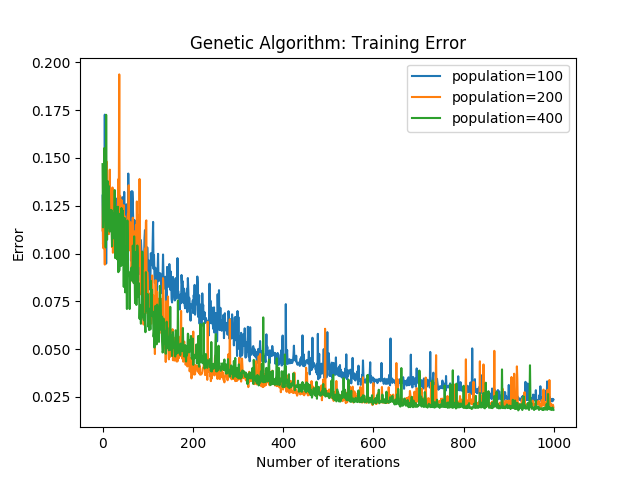
\includegraphics[width=\linewidth]{out/ga/population-training.png}
          \caption{Training error}
          \label{fig:ga-population-1}
        \end{subfigure}\hfil
        \begin{subfigure}{0.5\textwidth}
          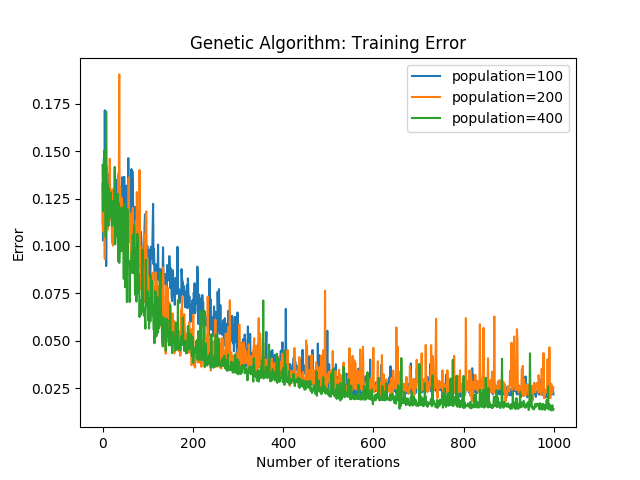
\includegraphics[width=\linewidth]{out/ga/population-testing.png}
          \caption{Testing error}
          \label{fig:ga-population-2}
        \end{subfigure}

        \caption{Learning curves for genetic algorithms with varying population size.}
        \label{fig:ga-population}
        \end{figure}

        TODO TODO

        \Fref{fig:ga-mating} shows the training and test error curves for the cancer data set using genetic algorithms for weight optimization, varying the number of organisms that mate in each generation.

        \begin{figure}[htb]
        \centering

        \begin{subfigure}{0.5\textwidth}
          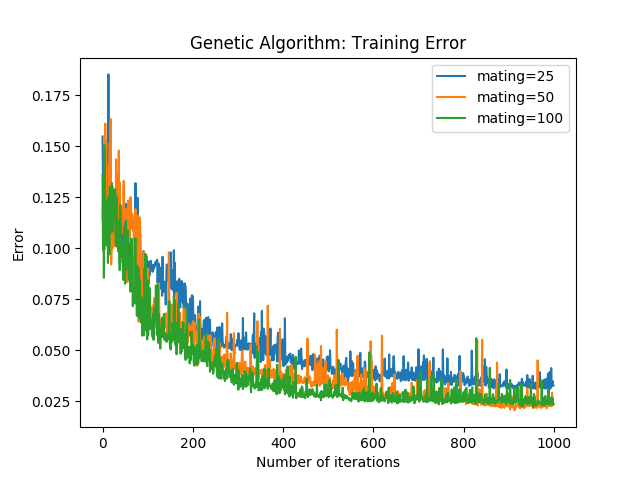
\includegraphics[width=\linewidth]{out/ga/mating-training.png}
          \caption{Training error}
          \label{fig:ga-mating-1}
        \end{subfigure}\hfil
        \begin{subfigure}{0.5\textwidth}
          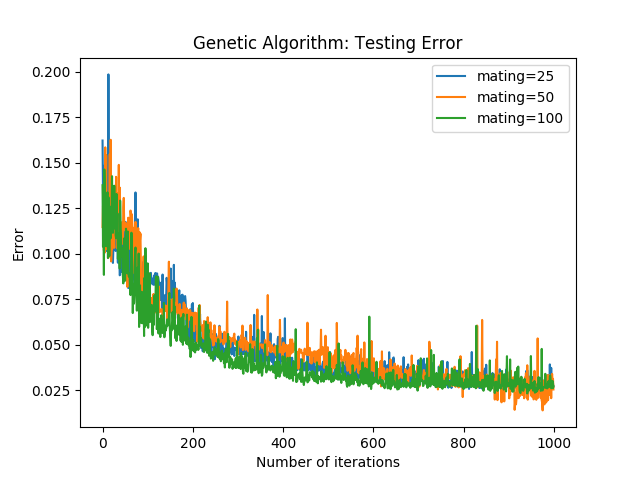
\includegraphics[width=\linewidth]{out/ga/mating-testing.png}
          \caption{Testing error}
          \label{fig:ga-mating-2}
        \end{subfigure}

        \caption{Learning curves for genetic algorithms with varying mating rates.}
        \label{fig:ga-mating}
        \end{figure}

        TODO TODO

        \Fref{fig:ga-mutation} shows the training and test error curves for the cancer data set using genetic algorithms for weight optimization, varying the number of organisms that mutate in each generation.

        \begin{figure}[htb]
        \centering

        \begin{subfigure}{0.5\textwidth}
          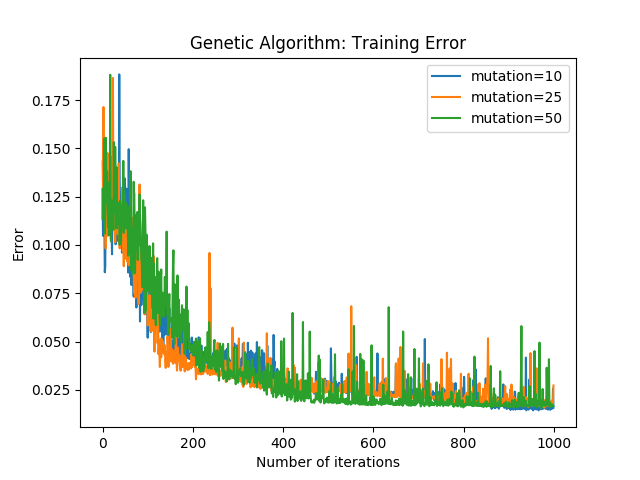
\includegraphics[width=\linewidth]{out/ga/mutation-training.png}
          \caption{Training error}
          \label{fig:ga-mutation-1}
        \end{subfigure}\hfil
        \begin{subfigure}{0.5\textwidth}
          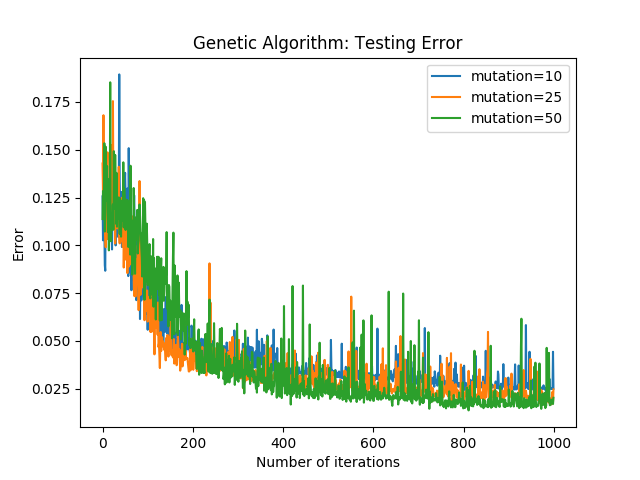
\includegraphics[width=\linewidth]{out/ga/mutation-testing.png}
          \caption{Testing error}
          \label{fig:ga-mutation-2}
        \end{subfigure}

        \caption{Learning curves for genetic algorithms with varying mutation rates.}
        \label{fig:ga-mutation}
        \end{figure}

        TODO TODO

        Finally selected population size of 400 first, then proportional mating and mutation rates. With a population size of 200, populations performed best with 25\% of the population mutating and 25\% of the population mating each generation.

      \subsubsection{Evaluation}
        \Fref{fig:ga-learning} shows the learning curves for the cancer data set using genetic algorithms.

        \begin{figure}[htb]
        \centering
        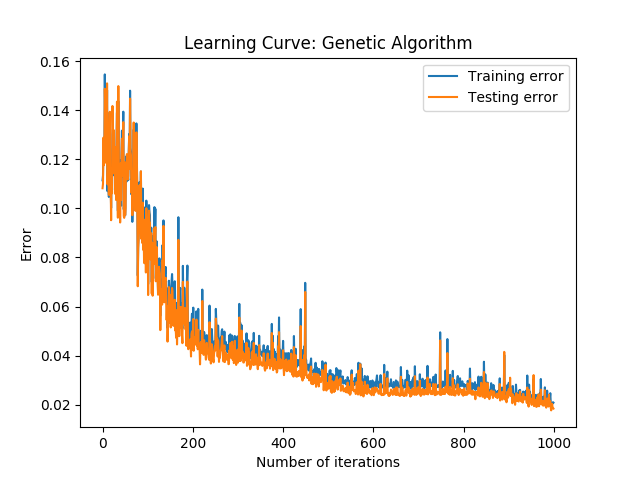
\includegraphics[width=.5\linewidth]{out/plot/GA.png}
        \caption{Learning curve for genetic algorithms.}
        \label{fig:ga-learning}
        \end{figure}

    \subsection{Comparison}
      After optimization of hyper-parameters, genetic algorithms slightly outperformed simulated annealing and randomized hill climbing after 1000 iterations. After the 1000th iteration, all search algorithms performed similarly, however, the genetic algorithm implementation minimized error at an earlier iteration than in the other two algorithms.

      However, this does not come without a cost. Genetic algorithms, while they did perform well, came at a wall clock time cost, training in a hefty 49.519 seconds as opposed to the 9.354 second and 8.976 second training time over 1000 iterations for randomized hill climbing and simulated annealing respectively. Because the genetic algorithm performed well, a lower number of iterations may be sufficient to improve the runtime of the genetic algorithm without compromising in accuracy, though this would require further tuning to ascertain.

      \Fref{fig:nn-compare} shows the training and test error curves for the cancer data set, using the optimized search algorithms for weight optimization that have been stated in this section.

      \begin{figure}[htb]
      \centering

      \begin{subfigure}{0.5\textwidth}
        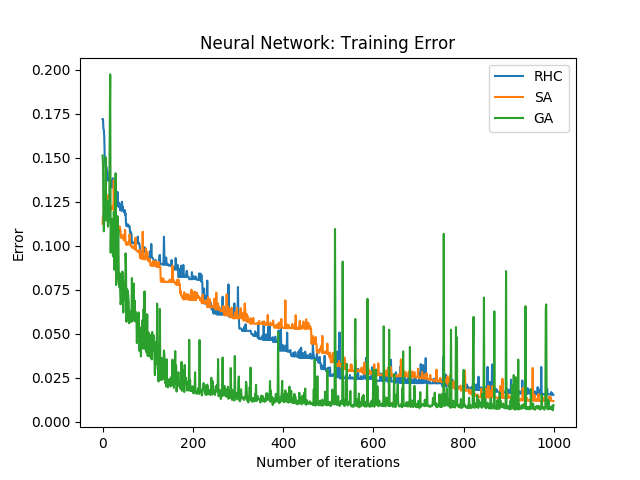
\includegraphics[width=\linewidth]{out/nn-combined-training.png}
        \caption{Training error}
        \label{fig:nn-compare-1}
      \end{subfigure}\hfil
      \begin{subfigure}{0.5\textwidth}
        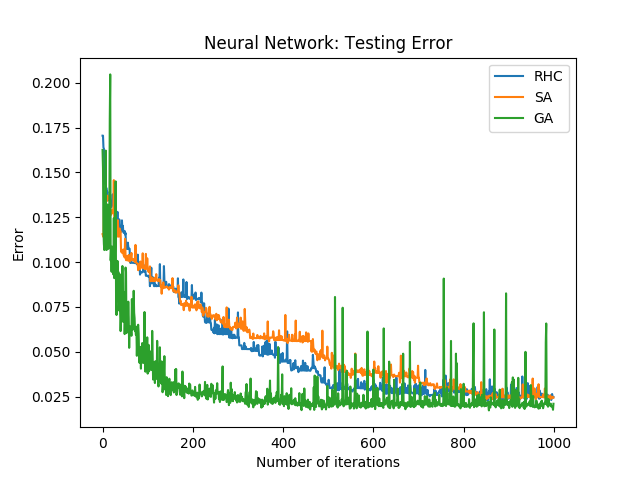
\includegraphics[width=\linewidth]{out/nn-combined-testing.png}
        \caption{Testing error}
        \label{fig:nn-compare-2}
      \end{subfigure}

      \caption{Learning curves for various weight optimization algorithms, with tuned parameters.}
      \label{fig:nn-compare}
      \end{figure}

  \section{Exploring Optimization Problems}
    Blah blah here are the ones I chose

    \subsection{Simulated Annealing}
      Here's a problem good with SA -- 

    \subsection{Genetic Algorithms}
      Here's a problem good with GA -- traveling salesman

    \subsection{MIMIC}
      Here's a problem good with MIMIC

  \section{Discussion}
    TODO

  \section{Conclusion}
    TODO

\end{document}